% Copyright 2004 by Till Tantau <tantau@users.sourceforge.net>.
%
% In principle, this file can be redistributed and/or modified under
% the terms of the GNU Public License, version 2.
%
% However, this file is supposed to be a template to be modified
% for your own needs. For this reason, if you use this file as a
% template and not specifically distribute it as part of a another
% package/program, I grant the extra permission to freely copy and
% modify this file as you see fit and even to delete this copyright
% notice. 

\documentclass{beamer}
\beamertemplatenavigationsymbolsempty

% path to graphics
\graphicspath{{img/}}

% write code
\usepackage{listings}
\usepackage{graphicx}
\usepackage{caption}
\usepackage[export]{adjustbox}
\usepackage{algorithm,algpseudocode}

% THEME
\usetheme{Frankfurt}

\title{Surface Remesher}

% A subtitle is optional and this may be deleted
%\subtitle{}

\author{Shayan Hoshyari}

\institute[University of British Columbia]{}

\date{December, 2016}

% subject for pdf file
\subject{CPSC524 Final Project}

% add some logo and stuff
% \pgfdeclareimage[height=1cm]{remesherlogo}{../image/logo.jpg}
% \logo{\pgfuseimage{remesherlogo}}

% Let's get started
\begin{document}

% ****************************************************************************
% *                             Title page
% ****************************************************************************
\begin{frame}[plain]
  \titlepage
\end{frame}

% ****************************************************************************
% *                             First Section
% ****************************************************************************

% ----------------------------------------------------------------------------
% -                              Goals
% ----------------------------------------------------------------------------

\begin{frame}[plain]{Surface Remeshing}
  
  Goal:
  \begin{itemize}
  \item \alert<2>{ Increase triangle quality       }
  \item \alert<2>{ Reduce/increase number of faces }
  \item Increase mesh regularity  
  \item Target based grading, e.g., curvature
  \end{itemize}

  \vspace{0.5cm}
  
  Main Constraint:
  \begin{itemize}
  \item \alert<2>{ Stay close to the initial surface }
  \end{itemize}

  \vspace{0.5cm}
  
  Based On:
  
  \begin{itemize}
    \item Vitaly Surazhsky, and Craig Gotsman. ``Explicit Surface Remeshing''
  \end{itemize}

\end{frame}

% ----------------------------------------------------------------------------
% -                              MaxPlanck
% ----------------------------------------------------------------------------
\begin{frame}[plain]{Surface Remeshing}

  \begin{figure}
    \includegraphics[width=0.8\textwidth]{../image/mp.png}
    \caption*{Max Planck model remeshed and coarsened.}
  \end{figure}

\end{frame}

% ----------------------------------------------------------------------------
% -                              Local Operations
% ----------------------------------------------------------------------------
\begin{frame}[plain]{Tools}

  Local operations in ``geodesic polar mapped space'':
  \begin{itemize}
  \item Edge collapse
  \item Edge split
  \item Edge flip
  \item Area based vertex relocation
  \item Laplacian smoothing  
  \end{itemize}

  \vspace{0.5cm}

  Keeping mesh fidelity:
  \begin{itemize}
  \item Fidelity error metrics to prevent certain operations
  \item Overlapping patchwise parameterization
  \end{itemize}
  
\end{frame}


% ----------------------------------------------------------------------------
% -                        Fidelity error metrics 
% ----------------------------------------------------------------------------
\begin{frame}[plain]{Fidelity Error Metrics}

  All created triangles $T$  with vertices $\mathcal V(T)$ must satisfy:
  
  \[\min( \vec N_i \cdot \vec N_j) > \cos(\theta_1) \quad i,j \in \mathcal V(T) \]
  
  \[\min( \vec N_i \cdot \vec N_T) > \cos(\theta_2) \quad i \in \mathcal V(T) \]

  \[ \theta_1 = \theta_2 = 20 \text{ deg} \]
  
\end{frame}

% ----------------------------------------------------------------------------
% -                        Geodesic Polar Mapping
% ----------------------------------------------------------------------------
\begin{frame}[plain]{Geodesic Polar Mapping}

  \begin{itemize}
  \item Map the neighborhood of an edge or vertex to two dimensions
  \item Vertex:
    \begin{itemize}
    \item Preserve distances
    \item Scale angles to sum to $2\pi$
    \end{itemize}
  \item Edge:
    \begin{itemize}
    \item Preserve angles
    \item Preserve distances  
    \item Rotate around common edge
    \end{itemize}
  \end{itemize}

  \begin{figure}
    \includegraphics[width=0.4\textwidth]{../image/geodesic.png}
  \end{figure}
  
\end{frame}


% ----------------------------------------------------------------------------
% -                         Overlapping patchwise parameterization
% ----------------------------------------------------------------------------
\begin{frame}[plain]{Overlapping Patchwise Parameterization}

  Output of local operations: $v =\text{Locate} (T,b), \quad T \in M$
  
  Possible Locate$()$ candidates:
  
  \begin{itemize}
  \item Using current mesh $M$
    \begin{itemize}
    \item $ v = \text{Interpolate} (T,b)$
    \end{itemize}    
  \item Projection on the initial mesh $M_0$:
    \begin{itemize}
    \item  $( (T_1,b_1), (T_2, b_2), (T_3, b_3) ) = \text{Reference} (T)$
    \item $ \hat{v}_i = \text{Interpolate}(\hat T_i, b_i) \quad
      i=1\ldots 3$
    \item  $ \hat T = \text{Triangle} (\hat v_1, \hat v_2, \hat v_3) $
    \item  $ \hat v = \text{Interpolate}(\hat T, b)$
    \item Find $\hat T_r$ where $\hat v = \text{Interpolate}( \hat
      T_r, b_r) $
    \item $ v =  \text{Interpolate}(T_r, b_r)$
    \end{itemize}
  \end{itemize}    

  \begin{figure}
    \includegraphics[width=0.8\textwidth]{../image/original_proj.png}
  \end{figure}

\end{frame}

% ----------------------------------------------------------------------------
% -                         Point Projection Comparions
% ----------------------------------------------------------------------------

\begin{frame}[plain]{Comparison of Projection Methods}

  \begin{figure}
    \begin{minipage}{0.32\textwidth}
      \centering
      \includegraphics[width=1\linewidth]{../image/horse_mouth_2.png}
    \end{minipage}
    %
    \begin{minipage}{.32\textwidth}
      \centering
      \includegraphics[width=1\linewidth]{../image/horse_mouth_0.png}
    \end{minipage} 
    % 
    \begin{minipage}{0.32\textwidth}
      \centering
      \includegraphics[width=1\linewidth]{../image/horse_mouth_1.png}
    \end{minipage}
    %
    \caption{Comparison of projection techniques}
  \end{figure}

\end{frame}

% ----------------------------------------------------------------------------
% -                            Patch Creation
% ----------------------------------------------------------------------------

\begin{frame}[plain]{Patch Creation}

  \begin{itemize}
  \item Find the patch using BFS search
  \item Check topology
  \item Trim ears
  \item Map to unit disk (CGAL)
  \end{itemize}
  
  \begin{figure}
    \begin{minipage}{.24\textwidth}
      \centering
      \includegraphics[width=1\linewidth]{../image/patch0.png}
    \end{minipage} 
    % 
    \begin{minipage}{0.24\textwidth}
      \centering
      \includegraphics[width=1\linewidth]{../image/patch1.png}
    \end{minipage}
    %
    \begin{minipage}{.24\textwidth}
      \centering
      \includegraphics[width=1\linewidth]{../image/patch2.png}
    \end{minipage} 
    % 
    \begin{minipage}{0.24\textwidth}
      \centering
      \includegraphics[width=1\linewidth]{../image/patch3.png}
    \end{minipage}
    %
  \end{figure}

\end{frame}

% ----------------------------------------------------------------------------
% -                     Area Based Vertex Relocation
% ----------------------------------------------------------------------------

\begin{frame}[plain]{Area Based Vertex Relocation}

  Area Based Vertex Relocation: Minimize $ \sum ( A_i(x,y) -
  \frac{1}{N} \sum A_i )^2 = 0 $

  \vspace{0.5cm}
  
  Laplacian Smoothing: $ v = \frac{1}{N} \sum v_i$

  \vspace{1cm}
  \begin{figure}
    \includegraphics[width=0.5\textwidth]{../image/area_0.png}
    \caption{Area Based Vertex Relocation}
  \end{figure}

\end{frame}

% ----------------------------------------------------------------------------
% -                        Global Algorithm
% ----------------------------------------------------------------------------

\begin{frame}[plain]{Global Algorithm}
  
\begin{algorithm}[H]
  \caption{Gluing the primitive operations together}
  %
  \begin{algorithmic}[1]
    
    \While{Target \# of vertices is reached}  
    \State Sort the edges according to ascending/descending adjacent
    triangle quality.
    \State Split/collapse the edges in the mentioned order. 
    \State Do not collapse or split edges that share an adjacent triangle.
    \State Perform 3 rounds of area based vertex relocation.
    \State Perform Dalauany edge flips.
    \EndWhile
    \State Optionally split all edges facing obtuse angles (not recursively).
    \State Do the following 10 times: 3 rounds of area based vertex relocation
    followed by Delaunay edge flips.
    \State Perform 10 rounds of Laplacian smoothing.
    %
  \end{algorithmic}
\end{algorithm}

\end{frame}

% ----------------------------------------------------------------------------
% -                             Simple Box
% ----------------------------------------------------------------------------

\begin{frame}[plain]{Sample Input}

  \only<1> {Input}
  \only<2> {Area based vertex relocation - iteration 1}
  \only<3> {Area based vertex relocation - iteration 2}
  \only<4> {Area based vertex relocation - iteration 3}
  \only<5> {Delaunay flips}
  \only<6> {Laplacian smoothing - iteration 1}
  \only<7> {Laplacian smoothing - iteration 2}
  
  \begin{figure}
    \only<1>{ \includegraphics[width=0.7\textwidth]{../image/sample_0.png} }
    \only<2>{ \includegraphics[width=0.7\textwidth]{../image/sample_1.png} }
    \only<3>{ \includegraphics[width=0.7\textwidth]{../image/sample_2.png} }
    \only<4>{ \includegraphics[width=0.7\textwidth]{../image/sample_3.png} }
    \only<5>{ \includegraphics[width=0.7\textwidth]{../image/sample_4.png} }
    \only<6>{ \includegraphics[width=0.7\textwidth]{../image/sample_5.png} }
    \only<7>{ \includegraphics[width=0.7\textwidth]{../image/sample_6.png} }
  \end{figure}
  
\end{frame}

% ----------------------------------------------------------------------------
% -                           Max Planck Model - 1 
% ----------------------------------------------------------------------------


\begin{frame}[plain]{Results}

  $N_v = 19132, 5000, 10000, 150000, 20000, 30000$

   \begin{figure}
    \begin{minipage}{.31\textwidth}
      \centering
      \includegraphics[width=0.7\linewidth]{../image/mpr_0.png}
    \end{minipage} 
    % 
    \begin{minipage}{0.31\textwidth}
      \centering
      \includegraphics[width=0.7\linewidth]{../image/mpr_a.png}
    \end{minipage}
    %
    \begin{minipage}{.31\textwidth}
      \centering
      \includegraphics[width=0.7\linewidth]{../image/mpr_b.png}
    \end{minipage} 
    % 
    \begin{minipage}{0.31\textwidth}
      \centering
      \includegraphics[width=0.7\linewidth]{../image/mpr_c.png}
    \end{minipage}
        %
    \begin{minipage}{.31\textwidth}
      \centering
      \includegraphics[width=0.7\linewidth]{../image/mpr_d.png}
    \end{minipage} 
    % 
    \begin{minipage}{0.31\textwidth}
      \centering
      \includegraphics[width=0.7\linewidth]{../image/mpr_e.png}
    \end{minipage}
    %
  \end{figure}

\end{frame}

% ----------------------------------------------------------------------------
% -                           Max Planck Model - 2
% ----------------------------------------------------------------------------
\begin{frame}[plain]{Results}
  
   \begin{figure}
    \begin{minipage}{.31\textwidth}
      \centering
      \includegraphics[width=1.0\linewidth]{../image/mp1.eps}
    \end{minipage} 
    % 
    \begin{minipage}{0.31\textwidth}
      \centering
      \includegraphics[width=1.0\linewidth]{../image/mp2.eps}
    \end{minipage}
    %
    \begin{minipage}{.31\textwidth}
      \centering
      \includegraphics[width=1.0\linewidth]{../image/mp3.eps}
    \end{minipage} 
    % 
    \begin{minipage}{0.31\textwidth}
      \centering
      \includegraphics[width=1.0\linewidth]{../image/mp4.eps}
    \end{minipage}
        %
    \begin{minipage}{.31\textwidth}
      \centering
      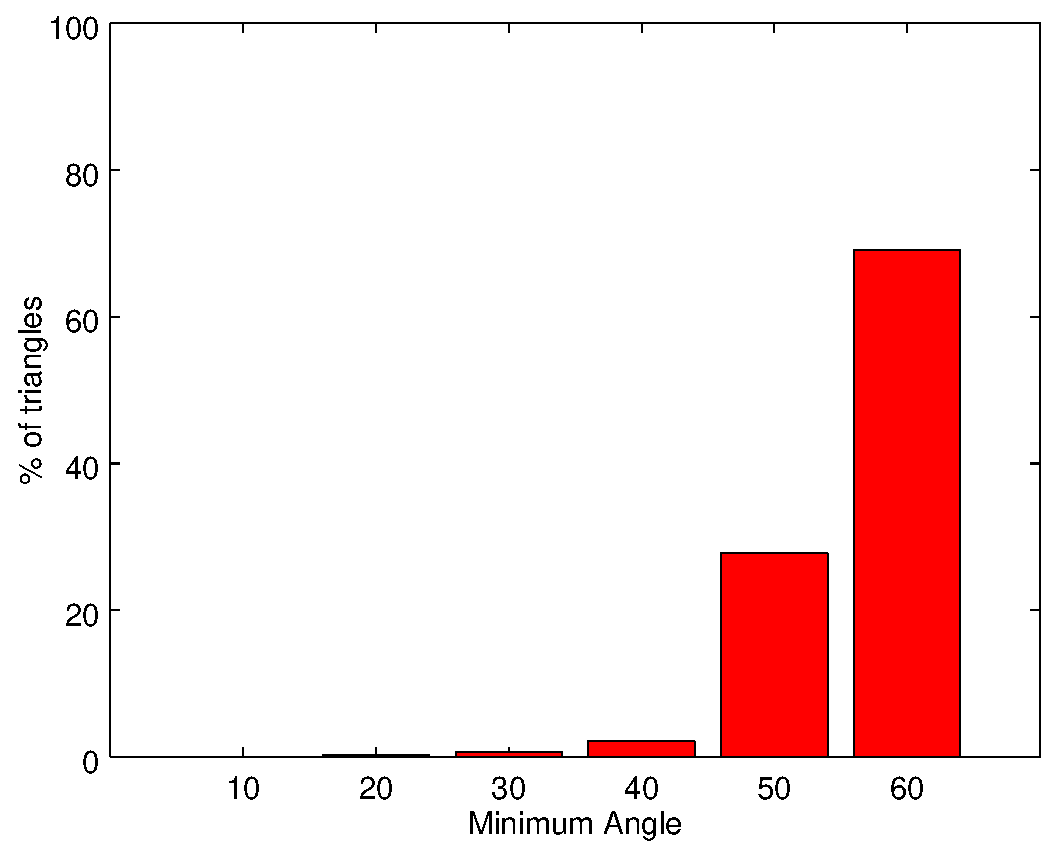
\includegraphics[width=1.0\linewidth]{../image/mp5.eps}
    \end{minipage} 
    % 
    \begin{minipage}{0.31\textwidth}
      \centering
      \includegraphics[width=1.0\linewidth]{../image/mp6.eps}
    \end{minipage}
    %
  \end{figure}


\end{frame}

% ----------------------------------------------------------------------------
% -                           Max Planck Model - 3
% ----------------------------------------------------------------------------
\begin{frame}[plain]{Results}
  
\begin{table}
  \begin{tabular}{cccc}
    %
    \hline
    Name &Vertex \# &Run Time &Patch \# \\
    \hline
    %
    % MAX_PLANCK
    %
    Initial &$19132$ &--- &--- \\
    %
    Case a &$5000$ &$7.94$ sec &$4568$ \\
    %
    Case b &$10000$ &$9.84$ sec &$4210$ \\
    %
    Case c &$15000$ &$11.14$ sec &$3984$ \\
    %
    Case d &$20000$ &$13.89$ sec &$3542$ \\
    %
    Case e &$30000$ &$22.32$ sec &$3520$ \\
    \hline
  \end{tabular}
\end{table}

\end{frame}

% ----------------------------------------------------------------------------
% -                           Possible Improvements
% ----------------------------------------------------------------------------

\begin{frame}[plain]{Possible Improvements}
  
  \begin{itemize}
  \item Using Bezier patches (PN triangles) to represent initial surface
  \item Adaptively subdividing areas with high initial fidelity error
  \item Goal based insertion and collapsing, e.g. regularization
  \item Curvature based grading
  \end{itemize}

\end{frame}


\end{document}
